\begin{figure}[tp]
\centering
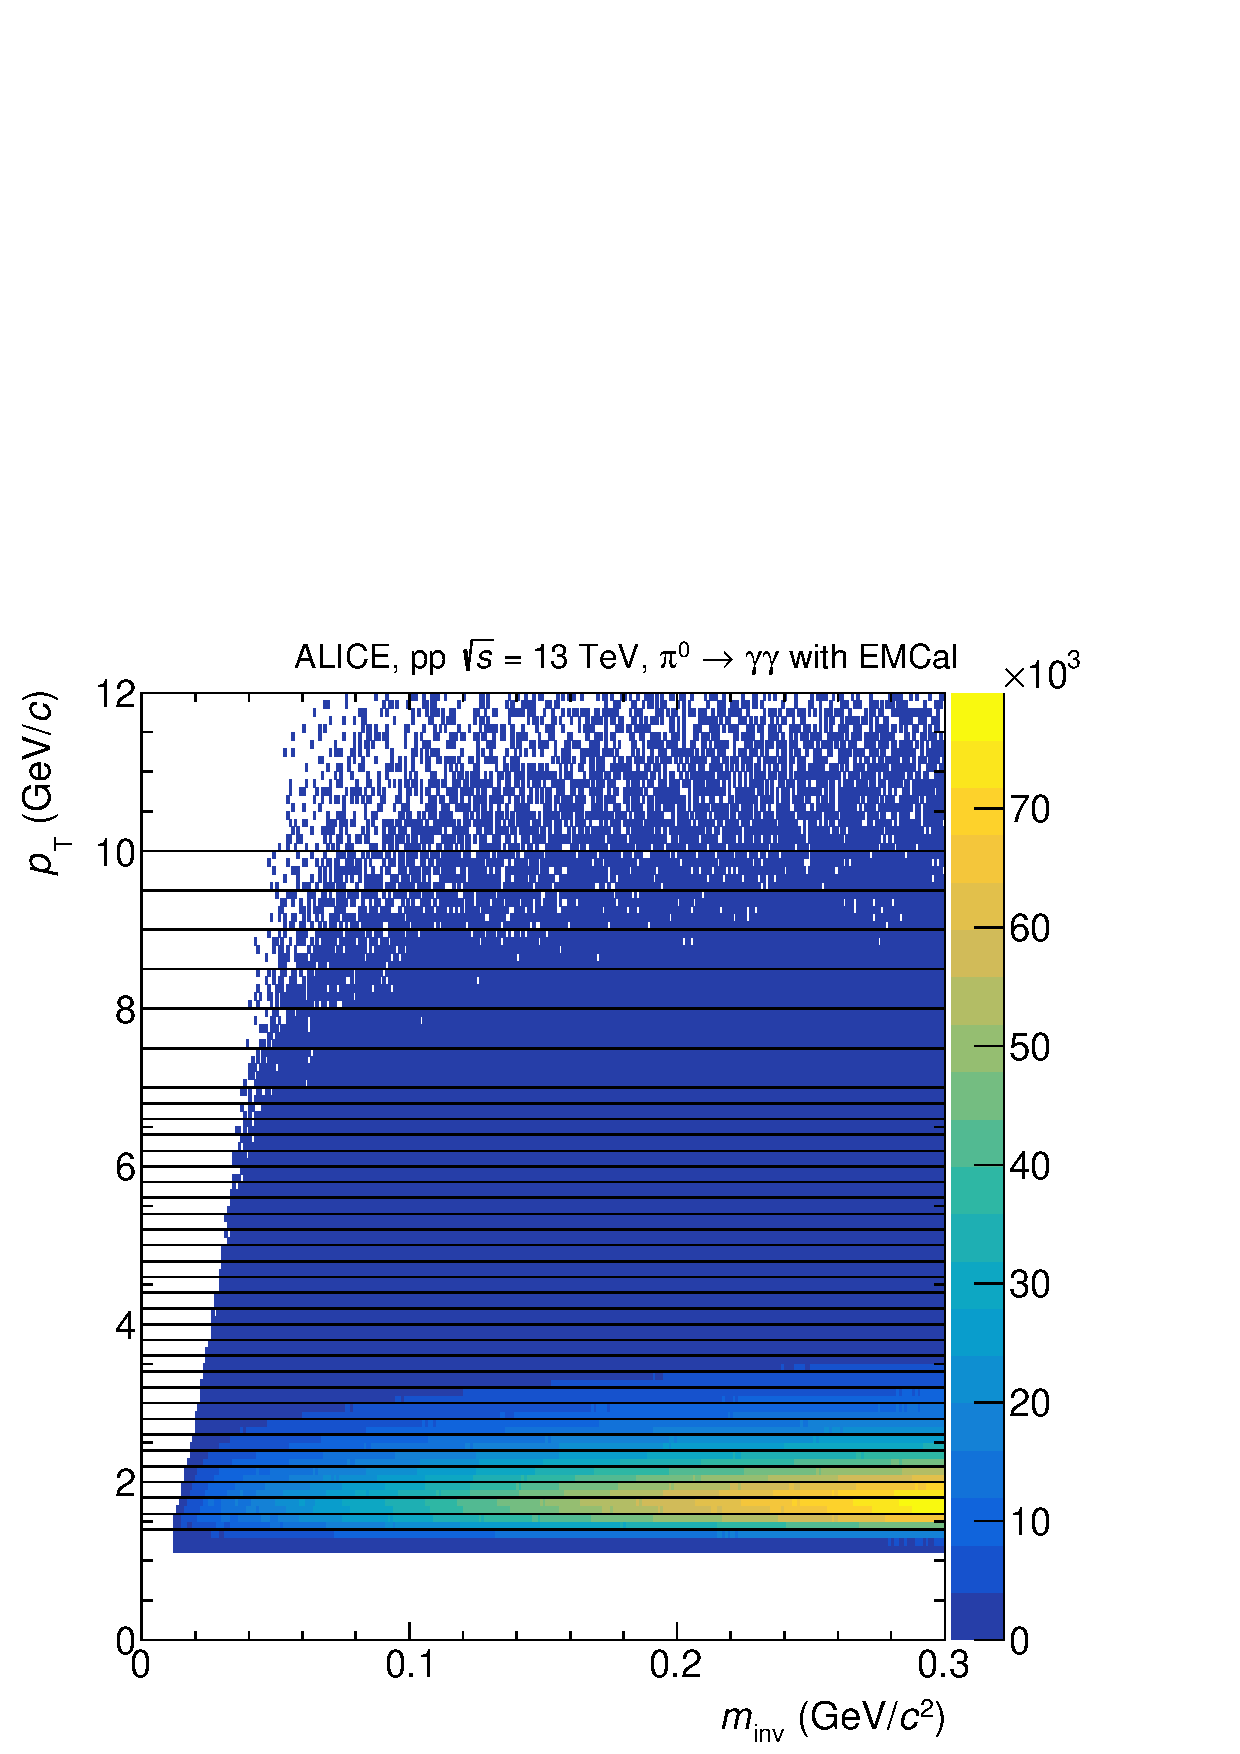
\includegraphics[width=.7\linewidth]{hInvMass_pT_Bkg.pdf}
\caption{$p_\text{T}$ und $m_\text{inv}$ als Funktion von der Anzahl von kombinierten  \textit{Clusterpaaren} aus unterschiedlichen \textit{events}.}
\label{figInvMassPt_b}
\end{figure}
Durch das paarweise Kombinieren aller Photonenkandidaten, wie es in Abschnitt \ref{s3s2} vorgestellt wurde, besteht ein großer Anteil der rekonstruierten Datenpunkte aus unkorreliert Paaren.
Um den unkorrelierten Untergrund abzuschätzen werden Photonenkandidaten aus unterschiedlichen \textit{events} paarweise miteinander kombiniert.
Dadurch wird sicher gestellt, dass zwischen den Photonenkandidaten keine Korrelation besteht.
Diese Methode wird als \textit{mixed event} Methode bezeichnet.
Abbildung \ref{figInvMassPt_b} zeigt eine Verteilung, bei der Photonenkandidaten aus unterschiedlichen \textit{events} miteinander kombiniert wurden.
Eine Häufung der Datenpunkte um eine bestimmte invariante Masse gibt es, wie zu erwarten, nicht.
Durch die Anforderungen an den Öffnungswinkel sind wieder keine Datenpunkte bei kleinen invarianten Massen zu finden.
Die untere Grenze der invarianten Masse, ab welcher Kombinationen möglich sind steigt mit $p_\text{T}$, analog wie zuvor bei Abbildung  \ref{figInvMassPt_a}.
\newline
In der \textit{mixed event} Methode gibt es eine größere Anzahl an Kombinationsmöglichkeiten, als in der \textit{same event} Methode.
Daraus resultiert eine größere Anzahl an Einträgen in der Verteilung der invarianten Masse und des Transversalimpulses, weshalb die Verteilung, die aus der \textit{mixed event} Methode kommt, skaliert werden muss an die Verteilung aus der \textit{same event} Methode.
Die Skalierung erfolgt bei $m_\text{inv} \in \left[0\,19,3\,0\right] (\text{GeV/}c^{2})$, da dort kein Signal erwartet wird.
Es ergibt sich für den Skalierungsfaktor:
\begin{align}
\label{eqBackSkalierung}
\alpha &= \frac{\sum_{i \neq j}\sum_{n}m_{\text{inv}}\left( \gamma^{(n)}_{i},\gamma^{(n)}_{j}\right) }{\sum_{i,j}\sum_{n \neq m}m_{\text{inv}}\left( \gamma^{(n)}_{i},\gamma^{(m)}_{j}\right) }
\end{align}
Die oberen Indize $m$ und $n$ stehen hierbei für ein Event, aus dem ein Photon kommt und die unteren Indize $i$ und $j$ numerieren die Photonen ($\gamma$).
\begin{figure}[tp]
\centering
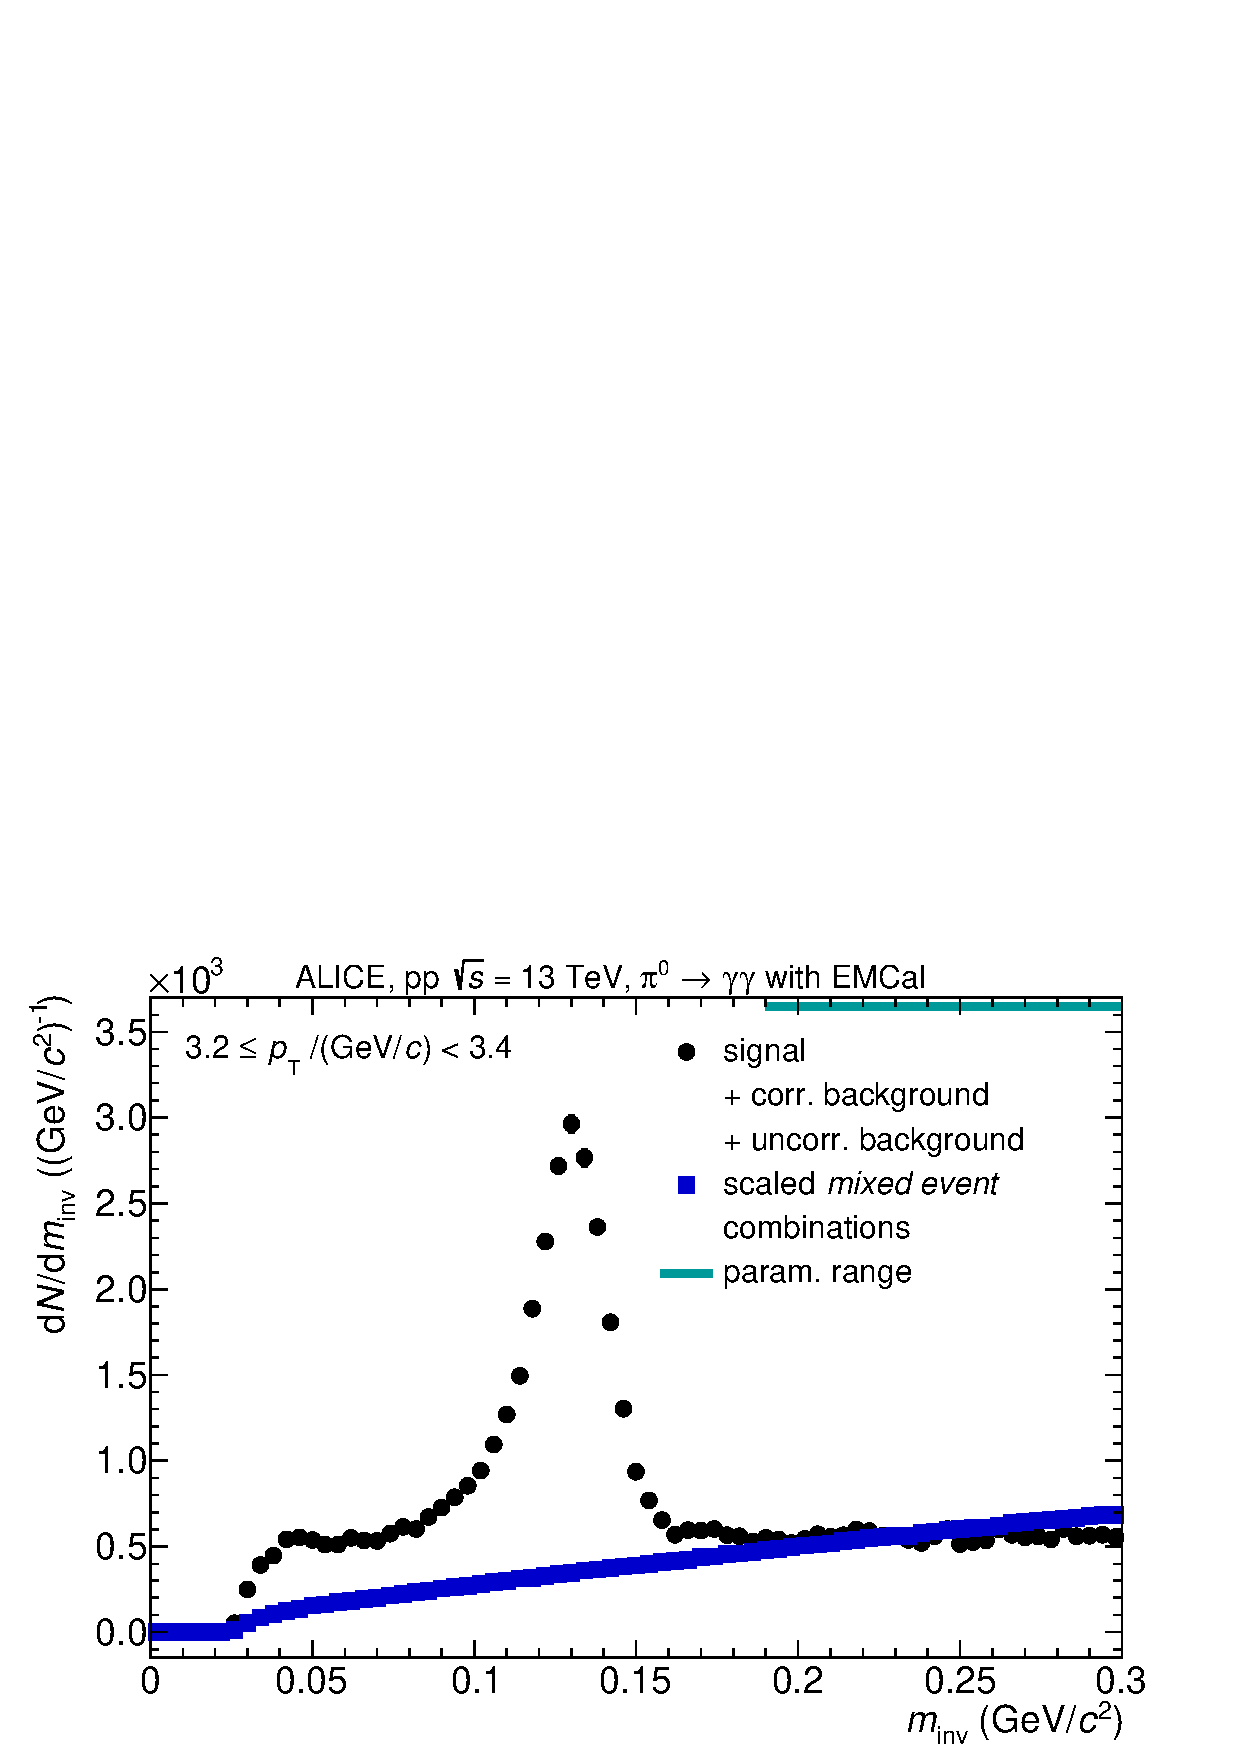
\includegraphics[width=.75\linewidth]{hUncorrBkgNorm.pdf}
\caption{Nach Gleichung \ref{eqBackSkalierung} skalierte {\it mixed event} Kombinationen als Abschätzung des unkorrelierten Untergrunds zusammen aufgetragen mit Signal zuzüglich beiden Untergrundkomponenten wie in Abbildung \ref{figSignalPlusBkg}.}
\label{figUncorrBkgNorm}
\end{figure}
\newline
Abbildung \ref{figUncorrBkgNorm} zeigt die skalierten \textit{mixed event} Kombinationen und das Signal zusammen mit dem korrelierten und dem unkorrelierten Untergrund.
Nachdem der unkorrelierte Untergrund abgeschätzt wird, wird dieser von der Verteilung der invarianten Masse aus der \textit{same event} Methode subtrahiert.
\begin{figure}[tp]
\centering
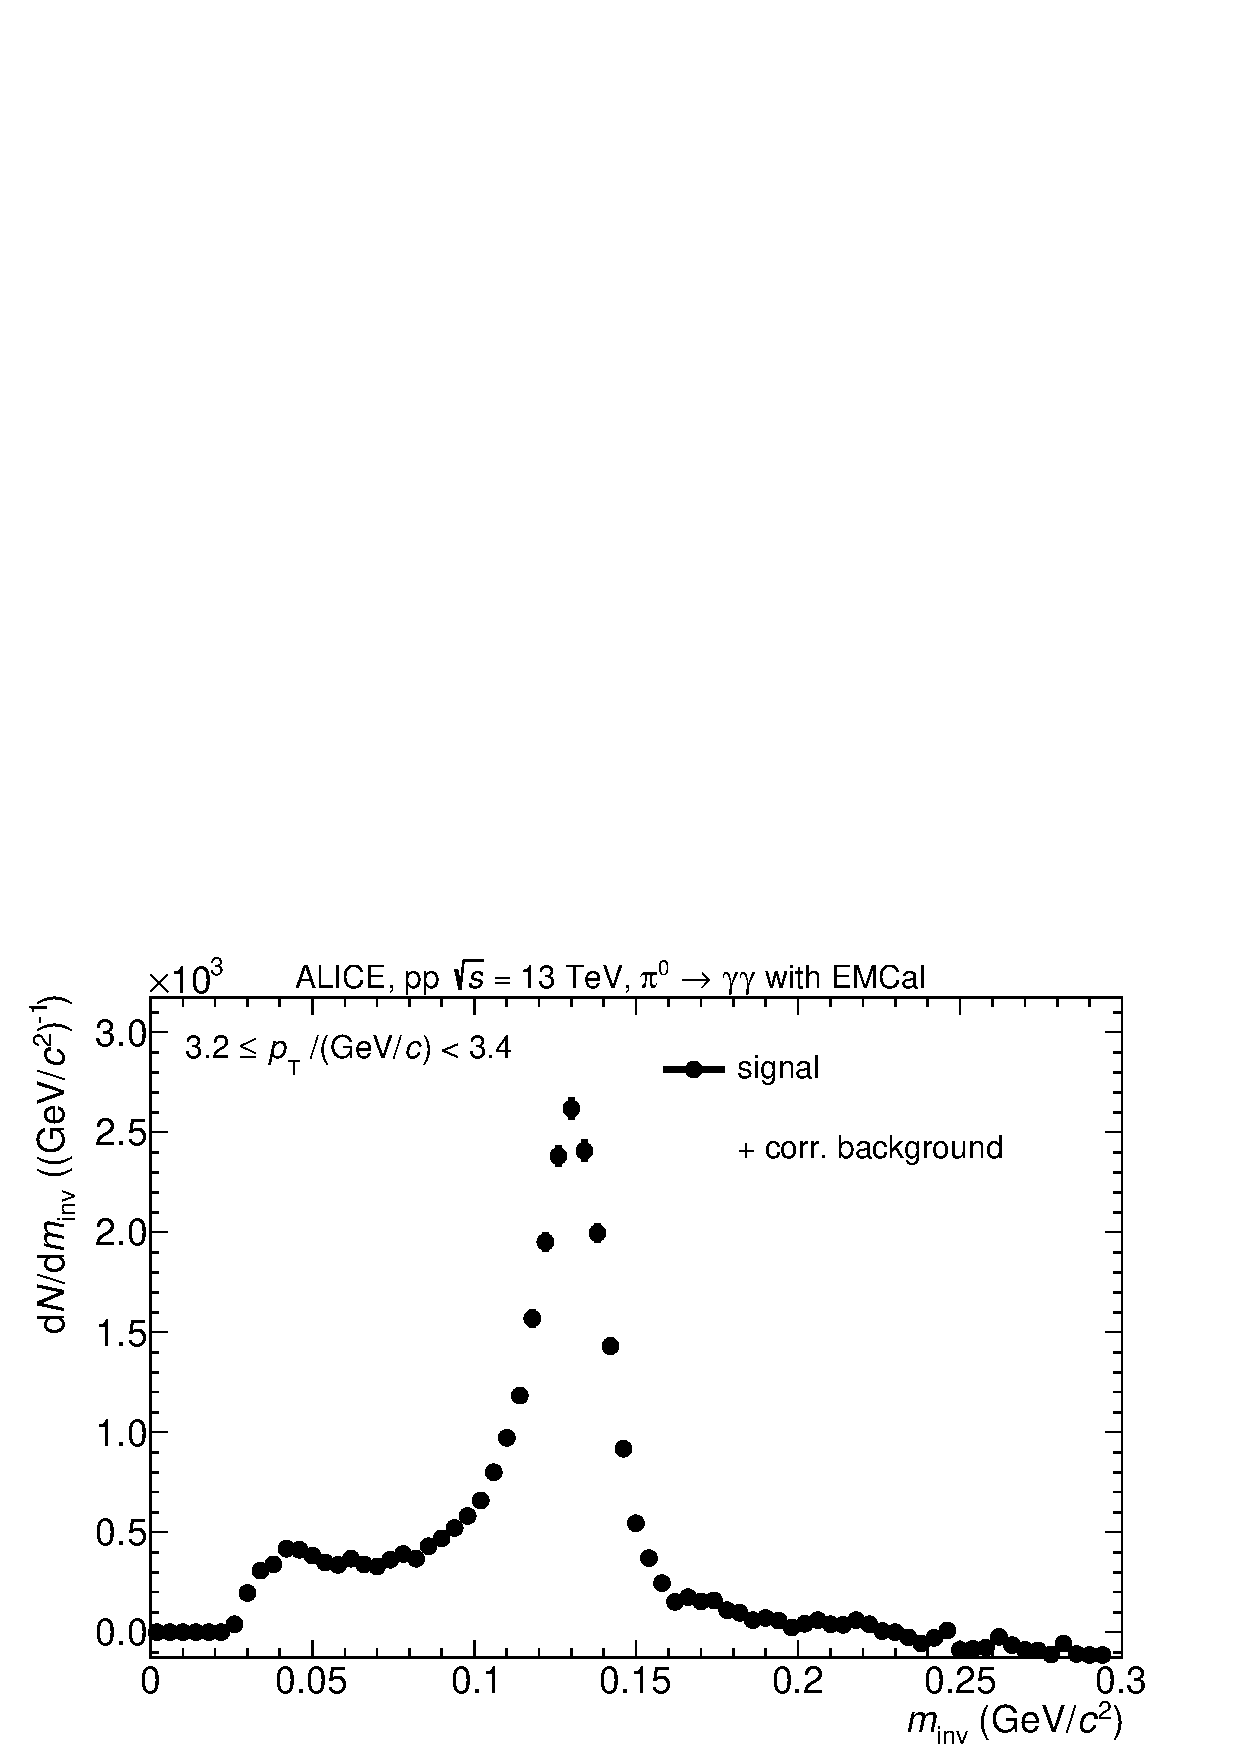
\includegraphics[width=.75\linewidth]{hInvMass_Data.pdf}
\caption{Signal nach Abzug des unkorrelierten Untergrunds.}
\label{figInvMass_Data}
\end{figure}
\newline
Abbildung \ref{figInvMass_Data} zeigt eine Verteilung der invarianten Masse aus der \textit{same event} Methode, nachdem die skalierten Kombinationen aus der \textit{mixed event} Methode, als Abschätzung der unkorrelierten Untergrunds, abgezogen wurden.
Durch die Subtraktion geht jegliche Information verloren, welche Photonenkandidatenpaare welchen Datenpunkt bilden.
Grund dafür ist, dass nicht einzelne Datenpunkte abgezogen werden, sonder lediglich eine gewisse Anzahl an Einträgen.
Deshalb spiegelt die Verteilung eine statistische Auswertung wider, mit statistischen Unsicherheiten.
\newline
Der nächste Schritt in der Analyse neutraler Pionen ist die Bestimmung des korrelierten Untergrunds.
Das Abschätzen mit einer linearen Funktion hat sich als gängigste Methode zur Abschätzung des korrelierten Untergrunds entwickelt und wird im Folgenden als Standardmethode bezeichnet.
In dieser Arbeit wird der korrelierte Untergrund sowie das reine $\pi^{0}$-Signal mit Hilfe von Monte Carlo Templates bestimmt.
Die Ergebnisse der Analyse mit Hilfe von Monte Carlo Templates, sowie mit der Standardmethode werden miteinander vergleichen, um eine Aussage über den möglichen Nutzen von Analysen mit Hilfe von Monte Carlo Templates treffen zu können.
Im folgenden Abschnitt wird zunächst die Standardmethode kurz erläutert.